\documentclass[a4paper, 10pt]{report}
\usepackage[italian]{babel}
\usepackage[T1]{fontenc}
\usepackage[utf8]{inputenc}
\usepackage{charter}
\usepackage{amsmath}
\usepackage{amsthm}
\usepackage{amsfonts}
\usepackage{graphicx}
\usepackage{wrapfig}
\usepackage{tcolorbox}
\usepackage{fancyhdr}
\usepackage{longtable}

\usepackage{geometry}
\geometry{a4paper, left=2cm,right=2cm,top=2cm,bottom=2cm}

\pagestyle{fancy}
\chead{}
\rhead{\bfseries 15 ottobre 2019}
\lhead{\bfseries Basi di dati}

\begin{document}
\begin{longtable}{| p{.15\textwidth} | p{.80\textwidth} |}
\textbf{Vincoli di cardinalità delle relazioni} & Data una relazione $R$ che coinvolge le entità $E_1, ..., E_n$, i vincoli di cardinalità si precisano per ogni entità $E_i$ che partecipa a $R$. Ogni vincolo di cardinalità precisa il numero minnimo e il numero massimo di istanze della relazione $R$ a cui un'istanza $E_i$ deve/può partecipare.

Un vincolo di cardinalità si rappresenta così: $(min, MAX)$

\begin{center}
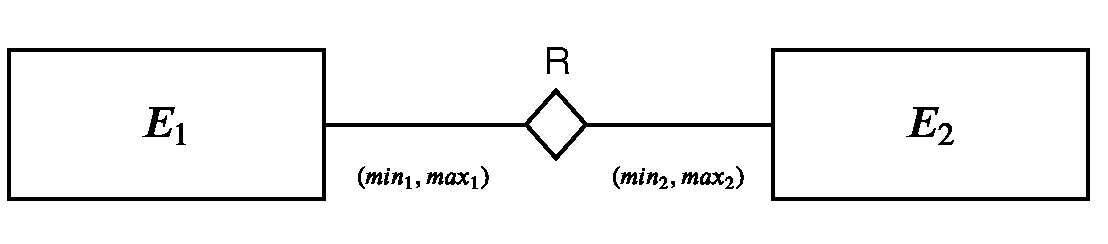
\includegraphics[scale=0.5]{img1.pdf}
\end{center}

I valori assumibili da $min$ sono:
\begin{itemize}
\item[-] $0$ -> indica che la relazione per le istanze di $E_i$ è opzionale;
\item[-] $1$ -> indica che la relazione per le istanze di $E_i$ è obbligatoria;
\item[-] $n > 1$ -> indica che ogni istanza di $E_i$ deve partecipare ad almeno $n$ istanze della relazione $R$.
\end{itemize}

I valori assumibili da $MAX$ sono:
\begin{itemize}
\item[-] $1$ -> al massimo un'istanza di $E_i$ partecipa ad una sola istanza della relazione $R$;
\item[-] $N$ -> indica che ogni istanza di $E_i$ può partecipare a più della relazione $R$;
\item[-] $n > 1$ -> indica che ogni istanza di $E_i$ può partecipare ad al massimo $n$ istanze della relazione $R$.
\end{itemize}

\underline{Esempio 1}:

\begin{center}
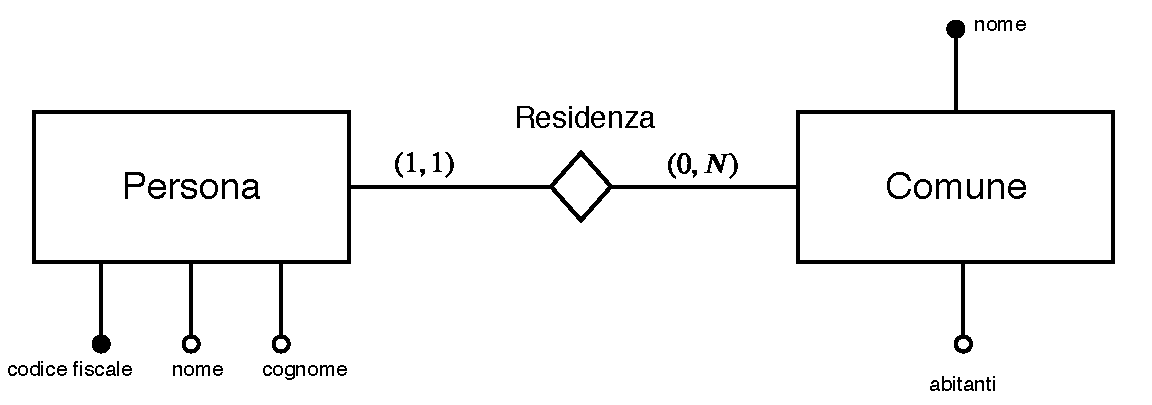
\includegraphics[scale=0.5]{img2.pdf}
\end{center}

Commenti all'esempio: $(1, 1)$ indica che una persona deve avere una residenza e che ogni persona può avere una sola residenza. Quindi, per ogni persona, la funzione residenza associa un solo comune (il comune deve essere già presente).
$(0, N)$ indica che posso istanziare comuni senza che esistano ancora le persone che ci abitano.

\underline{Esempio 2}: esercizio ER1 con vincoli di cardinalità

\begin{center}
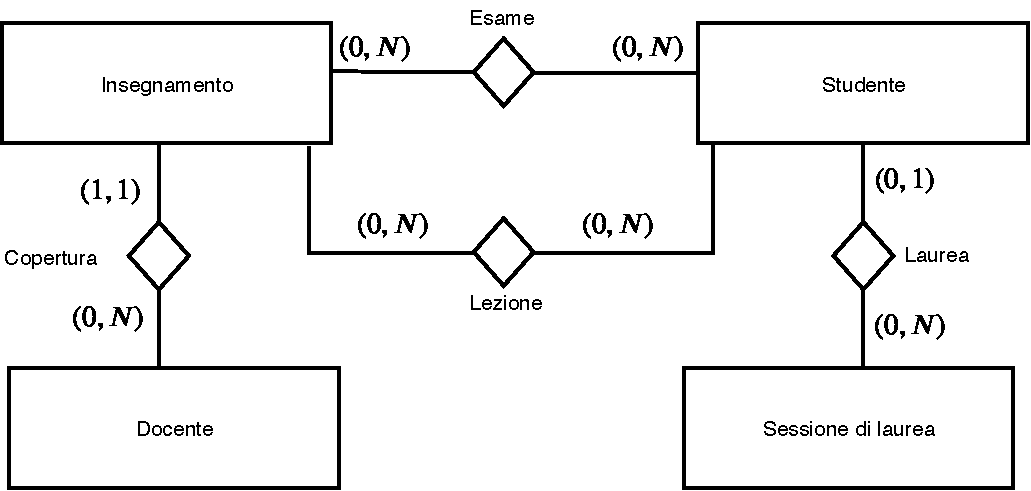
\includegraphics[scale=0.5]{15ottobre03.pdf}
\end{center}

Commenti all'esempio: essendo $min = 0$ in docente, posso inserire un docente quando voglio, mentre l'insegnamento può essere instanziato solo se esiste il docente.
\end{longtable}

\begin{tcolorbox}[title=\textbf{Esempio 1 in UML}]
\begin{center}
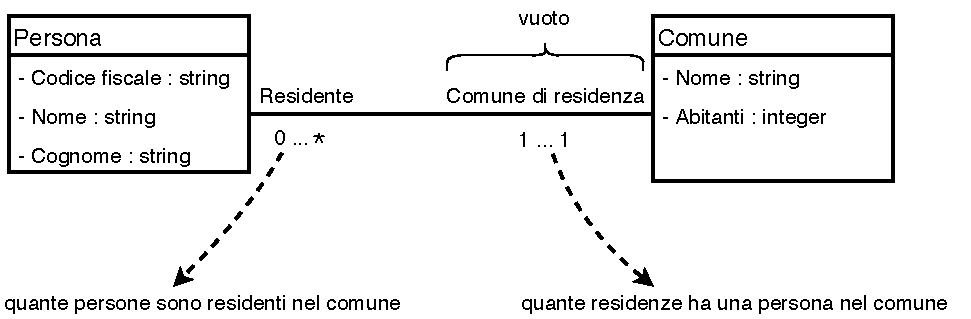
\includegraphics[scale=0.75]{15ottobre04.pdf}
\end{center}
\end{tcolorbox}

\begin{longtable}{| p{.15\textwidth} | p{.80\textwidth} |}
\textbf{Attributi opzionale e multivalore} & Gli aatributi opzionali/multivalore si creano precisando, su un normale attributo, una cardinalità diversa da $(1, 1)$, che  è la cardinalità di default.

Le cardinalità possibili per l'attributo sono:
\begin{itemize}
\item[-] $(0, 1)$ -> indica che l'attributo è opzionale;
\item[-] $(1, N)$ -> indica che l'attributo è multivalore;
\item[-] $(0, N)$ -> indica che l'attributo è opzionale e multivalore.
\end{itemize}

\begin{center}

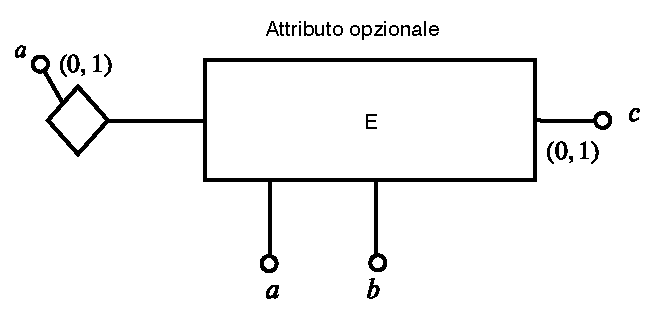
\includegraphics[scale=0.5]{15ottobre05.pdf}

(attributo opzionale)

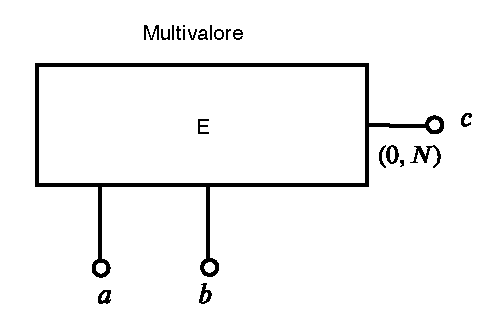
\includegraphics[scale=0.5]{15ottobre08.pdf}

(attributo multivalore)
\end{center}

\underline{Esempio}:

\begin{center}
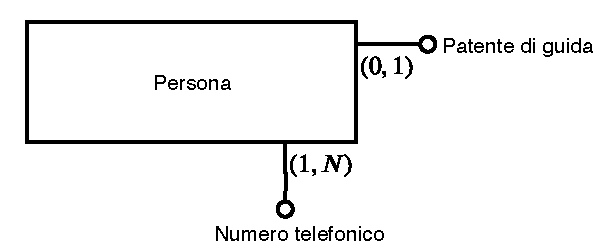
\includegraphics[scale=0.5]{15ottobre07.pdf}
\end{center}
\\
\textbf{Attributo composto} & Un attributo composto permette di raggruppare attributi con affinità di significato.

\underline{Esempio}:

\begin{center}
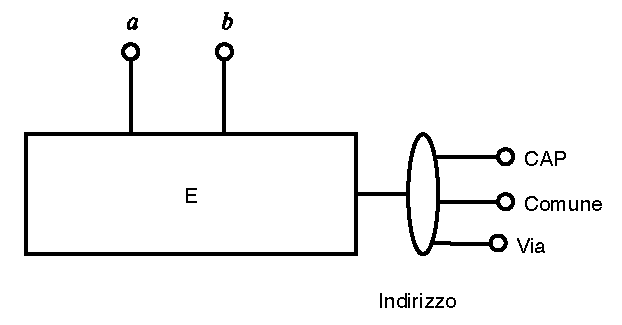
\includegraphics[scale=0.5]{15ottobre06.pdf}
\end{center}

\end{longtable}







\end{document}